\chapter{Results}
\label{chap:results}


\section{Hyperparameter gridsearch}

The extended search grid for the hyperparameters of the retrained SMILES models, along with the results from the gridsearch of MassSpecGym, can be found in table \ref{tab:gridsearch}.
The hyperparameter combination for which the trained model has lowest validation loss is denoted in bold.

\begin{table}[h]
	\caption{
		SMILES transformer, Gridsearch MassSpecGym vs Gridsearch from this Thesis (lowest validation loss models in bold)
	}
    \resizebox{\textwidth}{!}{
	\begin{tabular}{p{6cm}W{c}{4cm}W{c}{4cm}}
		\toprule
                \textbf{Hyperparams} & \textbf{MassSpecGym} & \textbf{Thesis Gridsearch} \\
            \midrule
                Learning Rate & $\mathbf{3\cdot 10^{-4}}, 1\cdot 10^{-4}, 5\cdot 10^{-5}$ & $1\cdot 10^{-3}, 3\cdot 10^{-4}, \mathbf{1\cdot 10^{-4}}$\\
                Batch Size & $512, \mathbf{1024}$ & $\mathbf{512}, 1024, 2048$ \\
                $n$ predictions & $\mathbf{10}$ & $\mathbf{10}$ \\
                Transformer hidden dimensionality & $\mathbf{256}, 512$ & $\mathbf{128}, 256, 512$ \\
                Number of attention heads & $\mathbf{4}, 8$ & $2, 4, \mathbf{8}$ \\
                Number of encoding layers & $\mathbf{3}, 6$ & $\mathbf{2}, 3, 4$ \\
                Number of decoding layers & $\mathbf{4}$ & $2, 3, \mathbf{4}$ \\
		\midrule
	\end{tabular}}
	\label{tab:gridsearch}
\end{table}

By retraining with the extended search grid, several models were found that outperformed the retrained model with the best hyperparameter combination from MassSpecGym, when comparing validation loss.
Note that the number of predictions is kept constant as this does not influence the loss.
The hyperparameters from the model with the lowest validation loss differ greatly from the retrained model from MassSpecGym. % 3 keer from?
Because the loss function does not accurately describe the model's ability to predict de novo molecules from \ac{MS/MS},
a naive sampler (that just iteratively samplers from the model's output distribution) was used to predict SMILES on the validation set.
The evaluation of the SMILES predictions from both models using this sampler can be found in figure \ref{fig:gridsearch_vs_paper}.
The MCES distance on the SMILES and tanimoto similarity on the converted fingerprints are calculated in the strict (top-1) and more relaxed (top-10) settings.

\begin{figure}[h]
    \centering
    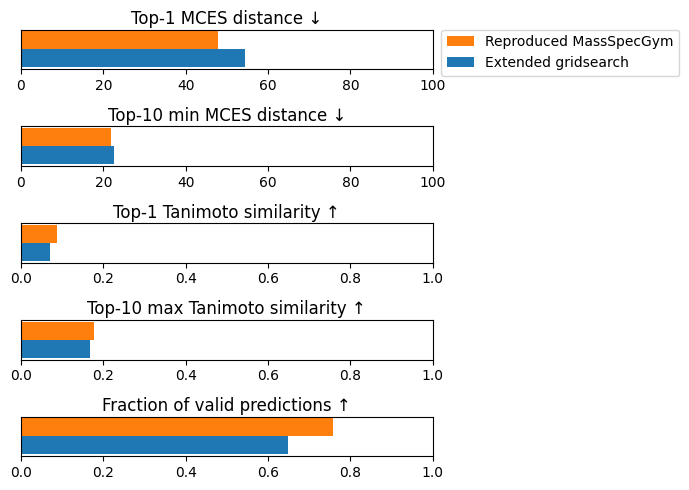
\includegraphics[width=0.6\textwidth]{figures/results/gridsearch_vs_paper.png}
    \caption{Performance comparison between the retrained SMILES model from the MassSpecGym paper versus the lowest validation loss SMILES model from the gridsearch, evaluated on the validation set}
    \label{fig:gridsearch_vs_paper}
\end{figure}

The top-1 and top-10 exact match accuracy for both models is (close to) zero.
Even though the naive sampler adds a bit of randomization by sampling from the output distribution, the retrained SMILES model from MassSpecGym outperforms the model with the lowest validation loss.

A big contributing factor to this performance difference is the fact that the retrained MassSpecGym model is able to predict 10\% more valid SMILES, as invalid SMILES have the maximum MCES distance and zero Tanimoto similarity.
The validity of the SMILES prediction can rely on the sampler and the temperature scaling of the output distribution.
Because only a naive sampler with no temperature scaling was used, it is possible that better performance can be extracted from these models using different samplers and temperature scaling.


\section{Samplers benchmark}

To test how much temperature scaling and different samplers can influence model performance, different samplers were used to predict the validation set of the model with the lowest loss from table \ref{tab:gridsearch}.
For this and all further experiments conducted in this thesis, the Tanimoto similarity is directly correlated to the MCES distance and will thus not be shown in the plots.
All performance differences shown with the MCES distance always show the same relative tanimoto similarities.

Firstly the temperature scaling influence is measured in figure \ref{fig:naive_and_greedy} for the top-1 and top-10 settings.
Because this will influence the randomness the sampler's predictions, a simple greedy sampler that always predicts the most likely token is shown as a deterministic baseline.
This sampler will always predict the same SMILES and can thus only be top-1 evaluated.

\begin{figure}[h]
    \centering
    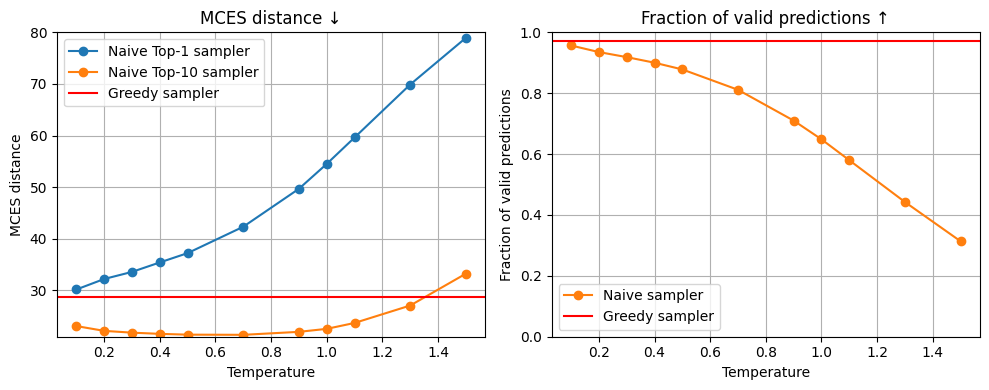
\includegraphics[width=1.0\textwidth]{figures/results/samplers/naive_and_greedy.png}
    \caption{Evaluation of the naive and greedy sampler on the validation set}
    \label{fig:naive_and_greedy}
\end{figure}

From figure \ref{fig:naive_and_greedy}, it is clear that the naive sampler performs poorly when only one prediction is evaluated (top-1).
Increasing the randomness (by increasing the temperature) for the top-1 naive sampler, only worsens the MCES distance.
As expected, the top-1 naive sampler MCES distance converges to the greedy sampler's MCES distance as the temperature approaches zero, as extremely low temperatures force the model to only predict the most likely token.

The top-10 naive sampler benefits greatly from its randomness, by performing better than the greedy sampler according to the MCES distance.
It shows to have an optimal temperature around $0.7$, for this SMILES model.
A higher temperature increases the randomness of the sampler too much causing the amount of valid predictions to drop.
A lower temperature starts to force the predictions towards the greedy sampler.
This shows that temperature can indeed influence the sampler's performance.

\subsection{Stochastic Samplers}

The randomness of the naive sampler can be tweaked using samplers such as top-k and top-p (nucleus sampling).
Because the stochastic samplers only benefit from their randomness when evaluating in a top-10 setting, only these results will be shown on the plots.
The temperature has shown to influence performance, therefore, a temperature search was conducted for each sampler with different parameters $k$ or $p$, where the optimal temperature (according to the lowest MCES distance) was selected.
This ensures that only the best results are shown for each the sampler with its parameter.
For completeness, the top-1, along with the temperature search results can be found in the appendix in section \ref{sec:sampler_full_results}.

\begin{figure}[h]
    \centering
    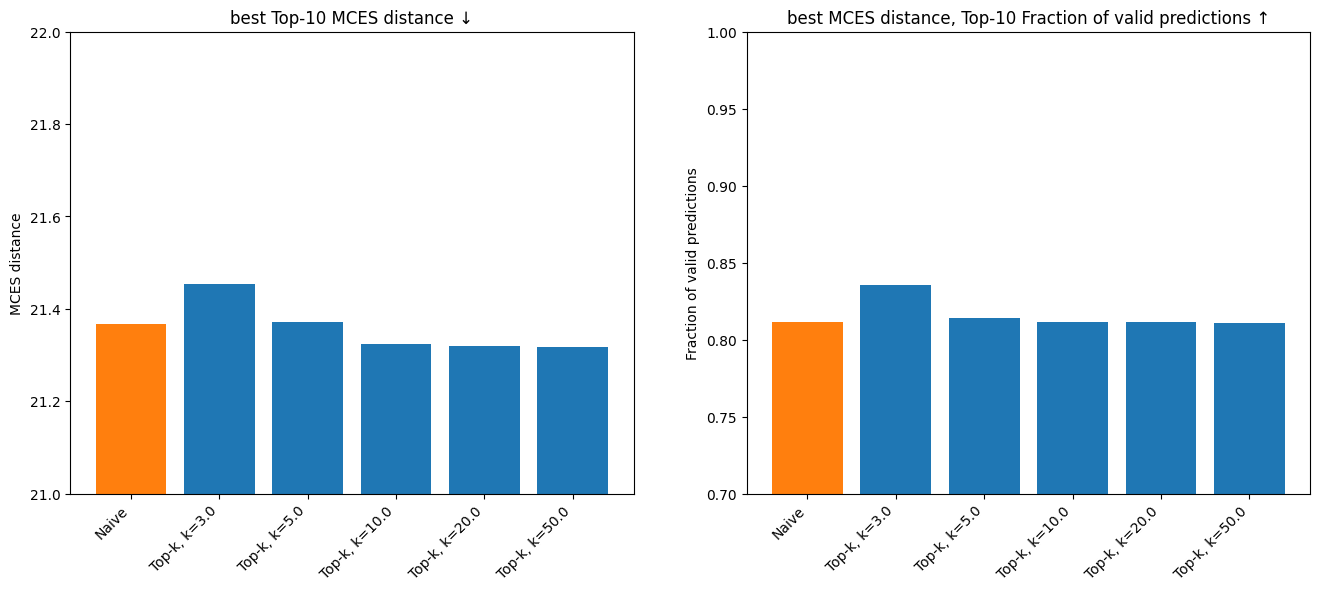
\includegraphics[width=1.0\textwidth]{figures/results/samplers/top-k.png}
    \caption{Evaluation of the (top-10, temperature optimized) top-k sampler and naive sampler on the validation set.}
    \label{fig:top-k}
\end{figure}

Figure \ref{fig:top-k} shows that top-k sampling can slightly improve performance when $k > 5$.
This shows that when the sampler gets forced with a low $k$ it performs slightly worse. 
Note that the y-axis is scaled for visibility, the improvement is very small.

\begin{figure}[h]
    \centering
    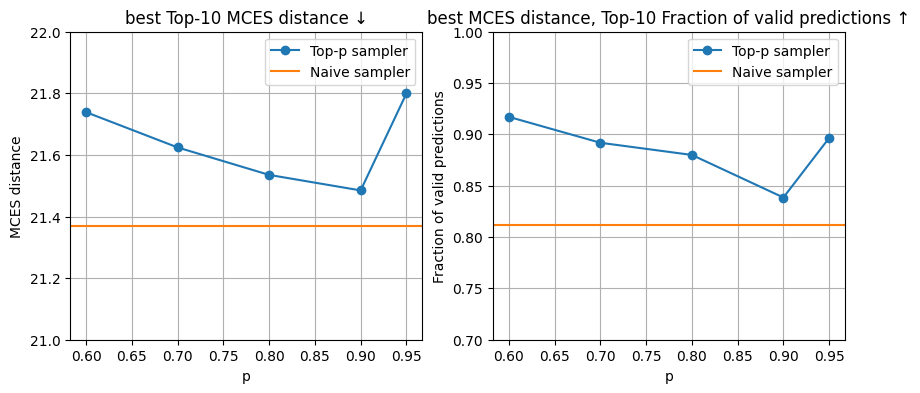
\includegraphics[width=1.0\textwidth]{figures/results/samplers/top-p.png}
    \caption{Evaluation of the (top-10, temperature optimized) top-p sampler and naive sampler on the validation set.}
    \label{fig:top-p}
\end{figure}

With top-k, limiting the randomization seems to slightly improve performance of the sampler, figure \ref{fig:top-p} shows that this does not hold for the top-p sampler.
Overall these randomization limiting samplers do not considerably improve the naive sampler.

The stochastic samplers seem to only benefit from the top-10 evaluation setting where the randomness of the sampler plays to its advantage.
The drawback of this method is the relatively low fraction of valid predictions.
Figure \ref{fig:naive_and_greedy} shows that in the temperature optimum still only $80\%$ of predictions are valid.
Because the top-10 setting only evaluates the best prediction, invalid predictions are not punished as long as there is one valid prediction for a spectrum.
These samplers are for this reason not suited for top-1 evaluation, where every invalid prediction is punished.

\subsection{Deterministic Samplers}

The beam search sampler is another deterministic sampler that improves upon the greedy sampler by increasing its search space to find optimal predictions.
Figure \ref{fig:beam-search} shows its performance for different search space sizes (beam widths).
The length regularization parameter $\alpha$ from the scoring function was also benchmarked for different beam widths but showed to have no influence on performance.
Only when large values were used ($\alpha > 10$), performance tanked to very poor results.
Forcing the sampler to predict longer token sequences with parameter $\alpha$ thus only hinders performance.

\begin{figure}[h]
    \centering
    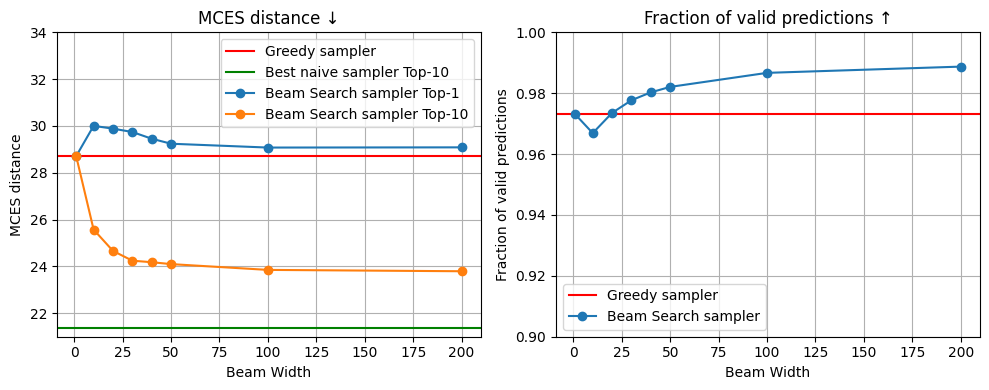
\includegraphics[width=1.0\textwidth]{figures/results/samplers/beam_search.png}
    \caption{Evaluation of the beam search sampler compared to the greedy and naive sampler on the validation set.}
    \label{fig:beam-search}
\end{figure}

Figure \ref{fig:beam-search} shows that the top-1 and top-10 MCES distance for the beam search sampler improves with increased search space as expected.
The spike in MCES distance and fraction of valid predictions on the first data point is because the beam width is 1, meaning it is essentially the same as the greedy sampler.
The top-10 beam search sampler outperforms the greedy sampler but does not come close to the best top-10 naive sampler results. 
For the top-1 setting, the performance shows to be worse than the greedy sampler.
This indicates that the scoring function is not optimal for extracting the correct molecular structure, especially with a small search space.
Because the top-10 evaluation outperforms the top-1, it shows that the prediction with the lowest score is often not the prediction with the lowest MCES distance, indicating the flaw of using the loss in the scoring function.
The only metric where the beam search sampler seems to outperform the others is the fraction of valid predictions.

These deterministic sampling methods perform best at predicting valid molecules as the fraction of valid predictions is substantially higher than with the optimal stochastic samplers.
When evaluating in a top-1 setting, where every invalid predictions is punished, these samplers are thus preferred.

Overall, from these results, the greedy sampler seems to perform best for the top-1 setting, while the naive sampler excels in the top-10 setting.
For all the following experiments in this thesis, the greedy and naive samplers are only used for the top-1 and top-10 setting respectively.

\section{\ac{BPE} as pretraining}

To measure the influence of the \acf{BPE} vocabulary computation of the tokenizer on the model's performance, SMILES models were trained with different tokenizers.
These tokenizers only differ in the vocabulary computation (and consequently, vocabulary size).
The training hyperparameters are kept the same for all models.

One simple tokenizer that does not pre-compute any patterns with \ac{BPE} in its vocabulary was used to train a baseline model.
The other tokenizers use datasets with different sizes of unlabeled SMILES from MassSpecGym.
These datasets are referred further as 4M for the 4,000,000 SMILES dataset, and 118M for the 118,000,000 SMILES dataset.
By using these unlabeled datasets, this could be considered a way to pre-train the model by storing frequently occurring patterns as one token in the vocabulary. 
All tokenizers, pre-computed with \ac{BPE}, also use the training SMILES in its \ac{BPE} corpus.
One tokenizer used \ac{BPE} with the training SMILES only to test how much unlabeled data can influence performance.

For the 4M and 118M dataset, a second tokenizer was pre-computed where the \ac{BPE} algorithm was given a more strict cut-off for grouping characters, by increasing the minimal frequency parameter from 2 (default value) to 10.
Lastly, because the vocabulary size of the 118M tokenizer reached the algorithm's threshold, a tokenizer was computed on the 118M dataset where computation halted as soon as the vocabulary reached the size of 5200 (= vocabulary size of the 4M tokenizer). 

Figure \ref{fig:bpe} shows the greedy top-1 and best naive top-10 samplers results of the models trained with these different tokenizers.
A new evaluation metric, the fraction of novel predictions, can be seen in the third plot.
It shows the fraction of valid predictions that are not present in the training set.
This measures how much the model is able to predict unseen SMILES as a metric to measure overfitting.
The complete temperature search for the naive top-10 sampler can be found in the appendix figure \ref{fig:bpe_appendix}.


\begin{figure}[h]
    \centering
    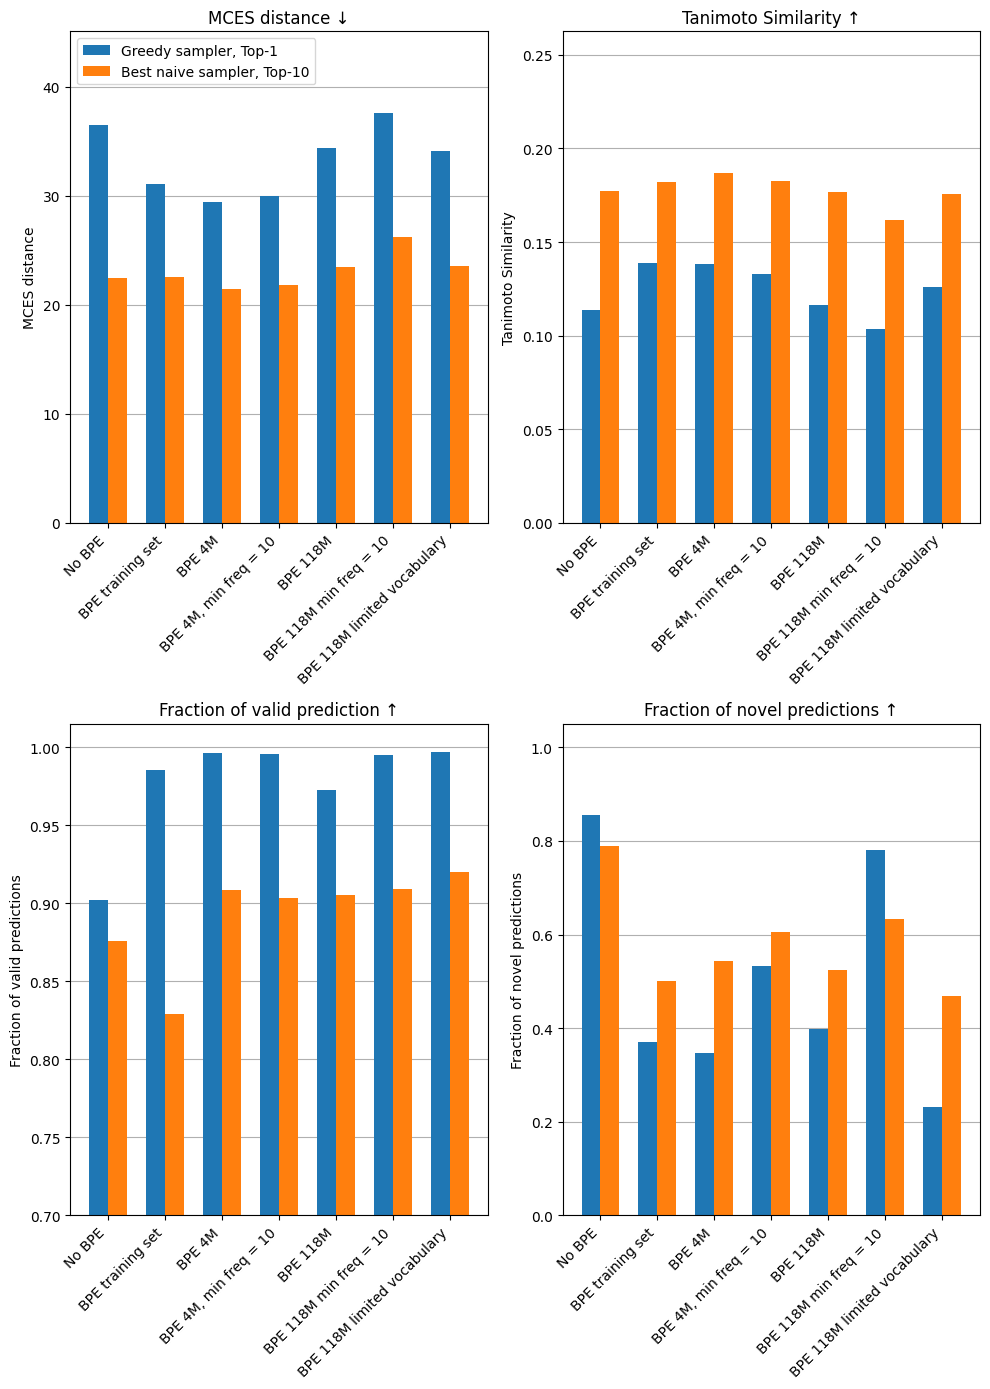
\includegraphics[width=1.0\textwidth]{figures/results/bpe_with_tanimoto.png}
    \caption{Evaluation on the validation set of SMILES models trained with different tokenizers}
    \label{fig:bpe}
\end{figure}

The most noticeable result from figure \ref{fig:bpe} is that the models that were trained using a BPE tokenizer have more valid predictions.
Note that the y-axis of the fraction of valid predictions plot does not start at zero for readability.
Using \ac{BPE} does indeed succeed in reducing invalid predictions.
A huge drawback, however, can be seen when looking ate the fraction of novel predictions.
Using \ac{BPE} with the standard parameters almost halves the number of novel predictions compared to the model trained with the tokenizer that did not use \ac{BPE},
and can thus directly be linked to the overfitting of the model.

The \ac{BPE} 4M tokenizer has the best performance looking at the MCES distance, it also achieves on of the highest number of valid predictions compared to the other tokenizers.
The poor amount of novel predictions does question if this result is due to overfitting as for the top-1 greedy sampler, $60\%$ of its predictions are from the training set SMILES.

A strange result is that the larger 118M dataset does not exceed the 4M tokenizer's MCES distance, more unlabeled data does not seem to help.
This can however be due to the fact that the quality of this dataset can be questioned.
Limiting the vocabulary size also shows to negatively impact the MCES distance, although for the 118M tokenizer it does increase the number of valid predictions.
Increasing the minimal frequency for patterns to be grouped also shows to noticeably increase the number of novel predictions.
This means that the overfitting trough \ac{BPE} models can be limited.
The 118M tokenizer with a minimal frequency of 10 almost reaches the same number of novel predictions as the model without \ac{BPE}, with $10\%$ more valid predictions for the top-1 greedy sampler.
Its MCES distance is worse however.

Overall, using \ac{BPE} with the tokenizers does reach its goal of improving the number of valid predictions.
When solely looking at the MCES distance, using \ac{BPE} can (in some cases) improve the model's performance.
The number of novel predictions does put these results in doubt, questioning the generalization of these models.

\section{Augmentation}

The influence of different augmentation methods was measured by retraining MassSpecGym's SMILES de novo model with different augmented datasets.
For each of these models, along with the baseline model without augmentation, the MCES distance, fraction of valid predictions and fraction of novel predictions were evaluated on the validation set.
Again, for the top-1 setting a greedy sampler was used and a temperature search of the naive sampler was performed for top-10.
Full results for the top-10 temperature searches can be found in the appendix at section \ref{sec:temp_search_appendix}.

\subsection{SMILES augmentation}

SMILES labels can be augmented by calculating the synonyms of these SMILES that represent the same molecular graphs.
The dataset can then be duplicated by copying the spectra and using the synonyms as labels.
This should allow the model to be more robust against repeated SMILES in the training set.
For this experiment three models were trained, for which the whole training set was duplicated once, twice and five times with SMILES synonyms (referred as 1x synonym, 2x synonyms and 5x synonyms respectively in the results).
For all these models the original training data with the original SMILES was kept in the training set.
Figure \ref{fig:smiles_augm} shows the evaluated results of these models using different evaluation metrics and settings.
The full naive sampler's top-10 temperature search results can be found in the appendix figure \ref{fig:smiles_augmentation_appendix}.

\begin{figure}[h]
    \centering
    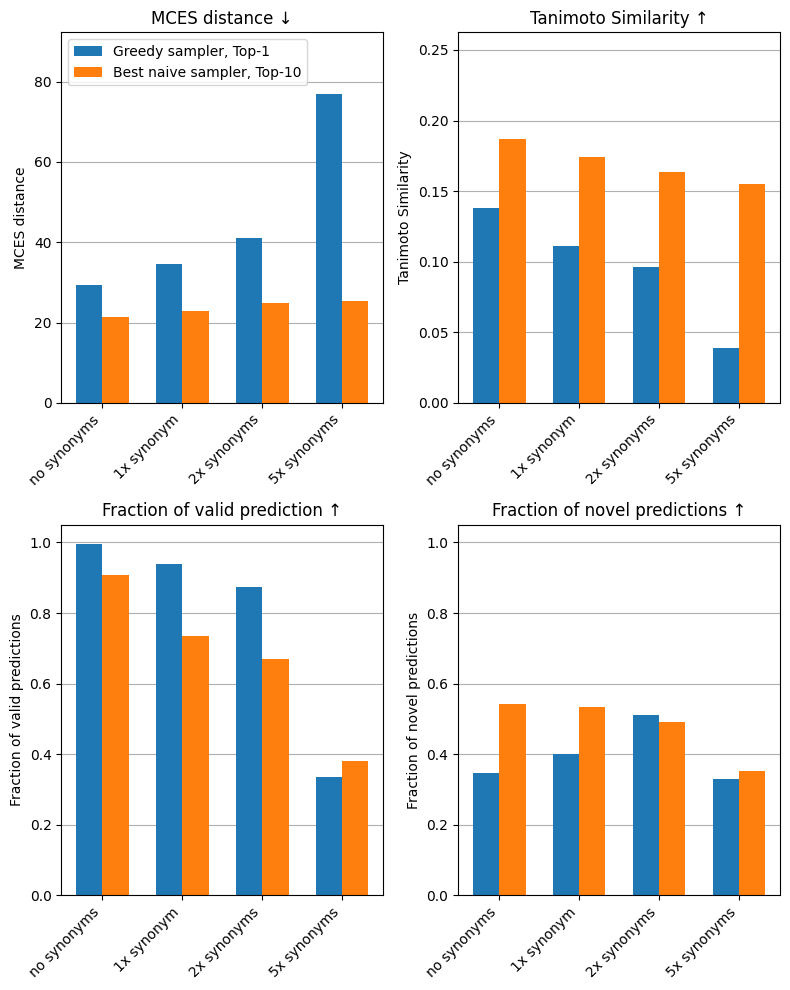
\includegraphics[width=0.8\textwidth]{figures/results/smiles_augmentation_with_tanimoto.png}
    \caption{Evaluation on the validation set of SMILES models trained with different SMILES augmented datasets}
    \label{fig:smiles_augm}
\end{figure}

From figure \ref{fig:smiles_augm} it is clear that SMILES augmentation does not seem to improve the de novo SMILES model from MassSpecGym.
The MCES distance and number of valid predictions get worse when more augmented SMILES are used for training.
Only the number of novel molecules, top-1 predicted, seems to increase by using some augmentation.
Too much augmentation reduces this again.

Overall, MassSpecGym's de novo SMILES model does not seem robust/powerful enough to handle any SMILES augmented data.

\subsection{Spectral augmentation}

By mimicking differing precursor masses from the input samples through spectral shifts, the input spectra can be augmented.
The dataset was augmented by applying random mz-shifts to spectra and copying their SMILES labels.
Two models were trained for this experiments, with $20\%$ and $100\%$ of the training spectra augmented (referred as $20\%$ mz shift augm. and $100\%$ mz shift augm. respectively in the results).
Again, the original training data is kept in the training set.
Figure \ref{fig:spectral_augm} shows the evaluated results of these models using different evaluation metrics and settings.
As usual, the full naive samplers top-10 temperature search results can be found in the appendix figure \ref{fig:spectral_augmentation_appendix}.

\begin{figure}[h]
    \centering
    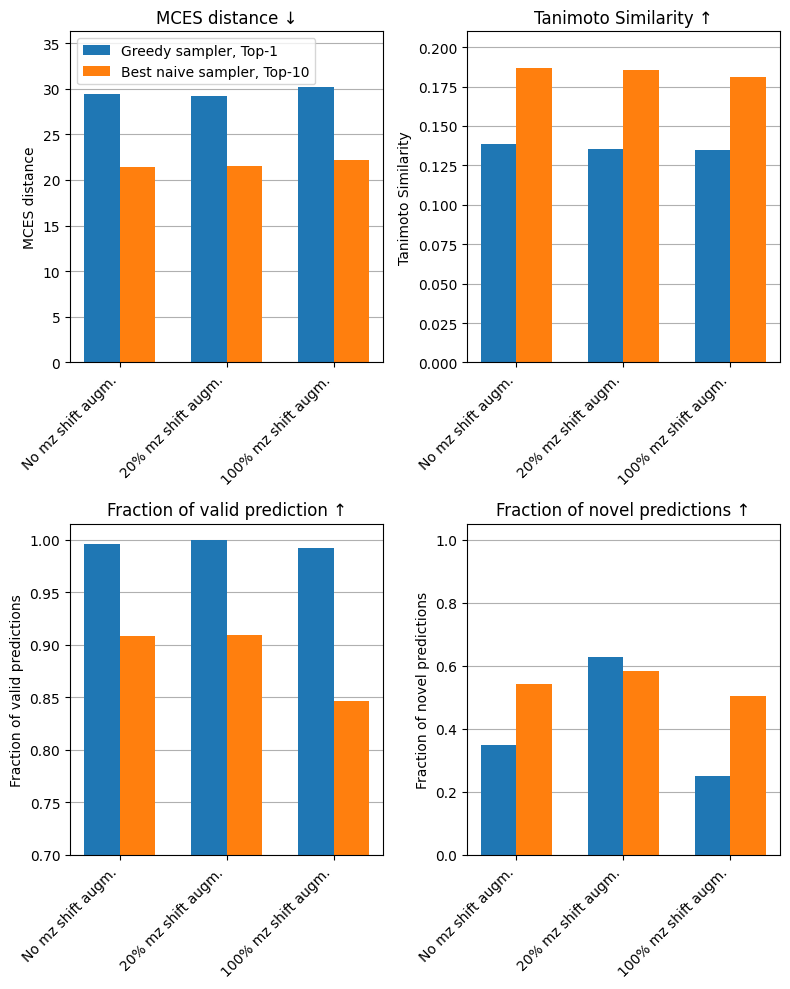
\includegraphics[width=0.7\textwidth]{figures/results/spectrum_augmentation_with_tanimoto.png}
    \caption{Evaluation on the validation set of SMILES models trained with different spectral augmented datasets}
    \label{fig:spectral_augm}
\end{figure}

In contrast to the previous augmentation method, the spectral augmentation does seem to help the de novo SMILES model from MassSpecGym.
While there are no significant improvements looking at the MCES distance, the $20\%$ augmented model is able to predict more valid and especially more novel molecules.
Too much augmentation, again, hinders performance as the original data gets drowned in augmented data.

This method of augmentation, when moderately used, clearly seems to help the model be less prone to overfitting, as the top-1 greedy sampler is able to predict more than $20\%$ more novel molecules. 

\section{Molecular representations benchmark}

Different molecular representations can be used to predict the structure of a molecule.
This experiment benchmarks the string-based molecular representations for the de novo structure prediction task.
InchIkey is the only representation discussed in section \ref{sec:molrepr} that is not used to train a model, as predicting hash keys is not possible.
All models were trained with the same hyperparameters.
Because tokenizers with vocabulary pre-computed with \ac{BPE} have shown to influence performance, for each molecular representation two models were trained.
One model used a Byte-pair encoded tokenizer, the other used a basic character tokenizer.
For all these models, a greedy sampler was used to evaluate the top-1 setting, while a temperature search was performed for the top-10 naive sampler.
Each molecular representation was thus evaluated four times.
The full results for the naive top-10 evaluation with the different temperatures can be found in the appendix figure \ref{fig:representations_appendix}.
Figure \ref{fig:representations} shows the MCES distance, fraction of valid predictions and fraction of novel predictions of the models trained on different molecular representations.

\begin{figure}[h]
    \centering
    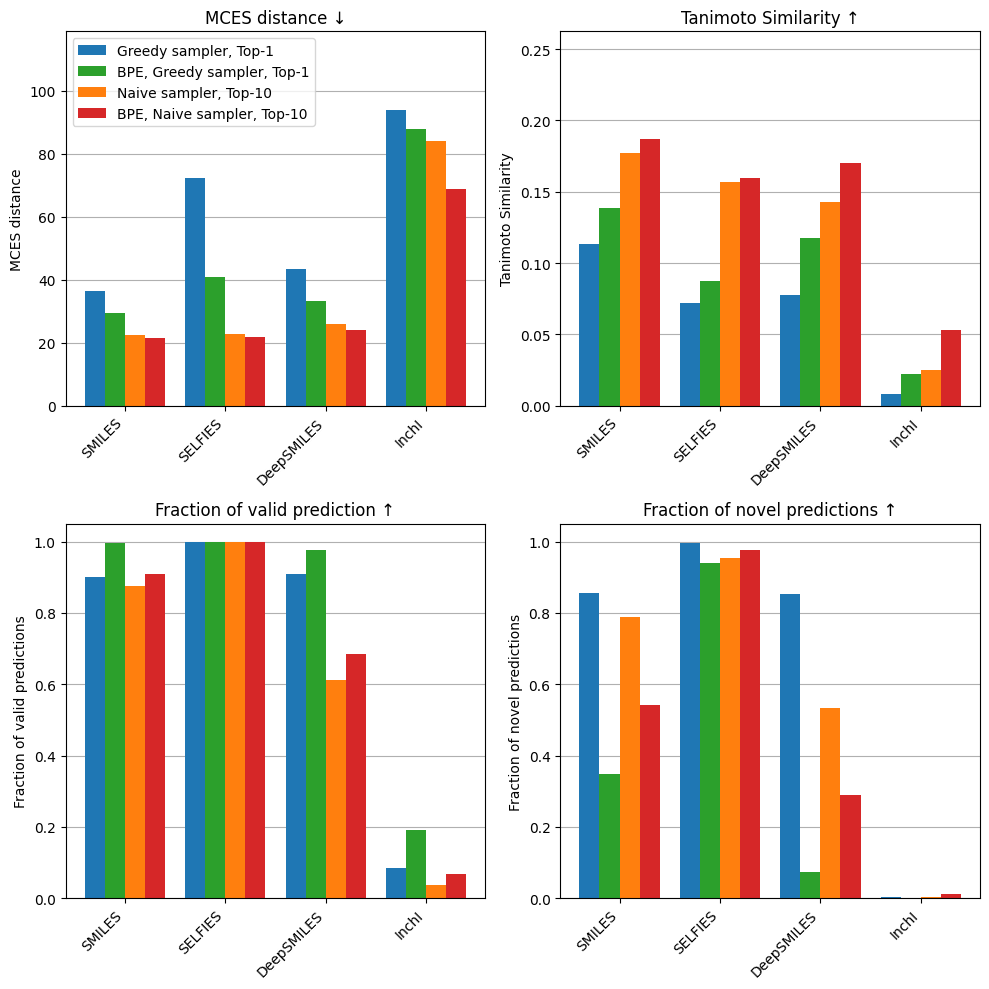
\includegraphics[width=1.0\textwidth]{figures/results/representations_with_tanimoto.png}
    \caption{Evaluation on the validation set of models trained with different molecular representations}
    \label{fig:representations}
\end{figure}

For the top-1 evaluation setting, SMILES outperforms the other molecular representations according to the MCES distance seen in figure \ref{fig:representations}.
SMILES and SELFIES seem to perform the best with top-10 evaluation, with their MCES distances being almost the same.
The models trained with SELFIES predicted the most valid predictions, as this is an inherent property of SELFIES, but noticeably also predicted the most novel molecules.
This indicates that the SELFIES models are less prone to overfitting on the training labels.

While DeepSMILES is closely related to SMILES with only slight modifications to reduce the chance of invalid predictions through syntax errors, it noticeably performs worse than SMILES, even having less valid predictions with top-10 evaluation.
The models trained using DeepSMILES are thus more prone to chemical errors as (almost) no syntax errors are possible.
An example of a prediction with a chemical error made by a DeepSMILES model can be seen in figure \ref{fig:invalid_pred}, where five bonds on one carbon atom are present, which is not possible in a stable environment.
The improvements DeepSMILES introduces over SMILES to combat invalid predictions for autoregressive generation seem to have the opposite results for de novo structure prediction, by introducing more chemical errors.
\begin{figure}[h]
    \centering
    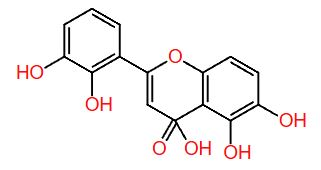
\includegraphics[width=0.5\textwidth]{figures/results/invalid_pred.JPG}
    \caption{2-dimensional representation of prediction with chemical error (SMILES: C1=CC=C(C(=C1C2=CC(=O)(C3=C(O2)C=CC(=C3O)O)O)O)O )}.
    \label{fig:invalid_pred}
\end{figure}

Out of the four representations benchmarked, InchI clearly shows to be the least fit for autoregressive generation, with most of its predictions being invalid.
This is caused by the fact that InchI has a strict layered structure to ensure its desired properties, which the models struggle to predict correctly.
When the model does succeed to predict an InchI with a valid syntax it almost always was present in the training set, showing heavy signs of overfitting.
To help the model understand the different layers of the InchI representation, a model was trained with a different decoder for each relevant layer. 
The results for this model can be found in the appendix figure \ref{fig:layered_inchi}.
This model was only able to predict a few valid predictions and struggled to synchronize the outputs of the different decoders.
The poor performance of InchI for this task is expected as the molecular representation was not designed for structure prediction.

The same conclusions from the \ac{BPE} experiment can be drawn for this experiment, where the use of a pre-computed vocabulary using \ac{BPE} improves the MCES distance and number of valid predictions but makes the model more prone to overfitting by having less novel predictions.
Only for the SELFIES top-10 evaluation, using \ac{BPE} also improves the number of novel predictions.

Overall, in this experiment, SMILES shows to be the best molecular representation when a top-1 evaluation is used.
Taking the amount of novel predictions into account, SELFIES performs the best for top-10 evaluation.
